\documentclass[tikz, border=5pt]{standalone}

\begin{document}
% \selectcolormodel{gray} %Makes everything monochrome
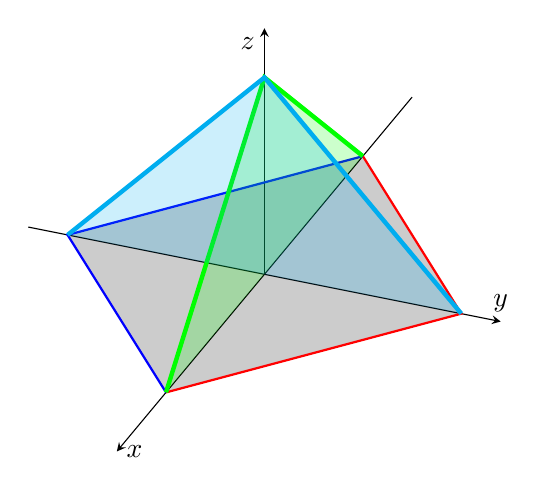
\begin{tikzpicture}[scale=2.5,x={(-5mm,-6mm)},z={(0,1cm)},y={(1cm,-.2cm)}]
  \draw [-stealth] (-1.5,0) -- (1.5,0,0) node [right] {$x$};
  \draw [-stealth] (0,-1.20,0) -- (0,1.20,0) node [above] {$y$};
  \draw [-stealth] (0,0,0) -- (0,0,1.25) node [below left] {$z$};
  
  \draw[fill=black,opacity=.2] (-1,0,0)--(0,-1,0)--(1,0,0)--(0,1,0);
  \draw[thick, red] (1,0,0)--(0,1,0) -- (-1,0,0);
  \draw[thick, blue] (1,0,0)--(0,-1,0) -- (-1,0,0);
  \draw[ultra thick,green, fill = green, fill opacity = 0.2] (1,0,0) -- (0,0,1) -- (-1,0,0);
  \draw[ultra thick, cyan, fill = cyan, fill opacity = 0.2] (0,1,0) -- (0,0,1) -- (0,-1,0);

  % \draw[fill=black,opacity=.2] (0,1,0)--(0,0,1)--(1,0,0);
  % \draw[fill=black,opacity=.5] (0,1,0)--(0,0,1)--(-1,0,0);
  \path ( 0, 0, 1) node[draw=none,fill=none,above,left]{}
        (-1, 0, 0) node[draw=none,fill=none,right] {}
         (1, 0, 0) node[draw=none,fill=none,below=0.5em,right] {}
         (0,-1, 0) node[draw=none,fill=none,left,above] {}
         (0, 1, 0) node[draw=none,fill=none,right,below=0.2em] {} ;
\end{tikzpicture}
\end{document}
